\documentclass{beamer}
\usetheme{Singapore}
\usepackage{hyperref}

\setbeamercolor{footnote mark}{fg=blue}
\setbeamerfont{footnote}{size=\tiny}
\setbeamerfont{caption}{size=\tiny}

\title{\textbf{Locating the Safest Apartments in Chicago}}
\subtitle{MACS 30122 Winter 22\\Final Project}

\author{Chongyu Fang, Feihong Lei, Zhennuo Wu, Jiachen Yu \thanks{We thank Dr. Nardin for her help and suggestions along the process of making this project possible. All errors are our own.}}
\institute{The University of Chicago}
\date{Mar 9, 2022}


\begin{document}
	\maketitle
	
\begin{frame}{Outline}
    \tableofcontents
\end{frame}


\section{Introduction}

\begin{frame}
	\frametitle{Rent and Crime Data Visualization Project}

	\begin{columns}
		\begin{column}{0.5\textwidth}
			\begin{itemize}
				\item Backgrounds:
				\begin{itemize}
					\item Accessing multiple websites for rental data and local crime rate
					\item Lack of crime information around properties on the rental website
					\item Credibility of data source
				\end{itemize}
				\item Purpose of this project:
				\begin{itemize}
					\item Aggregated rental data and crime rate data visualization via heat map
					\item User-friendly Interface
				\end{itemize}
			\end{itemize}
		\end{column}
	
		\begin{column}{0.5\textwidth}
			\begin{figure}[H]
				\centering
				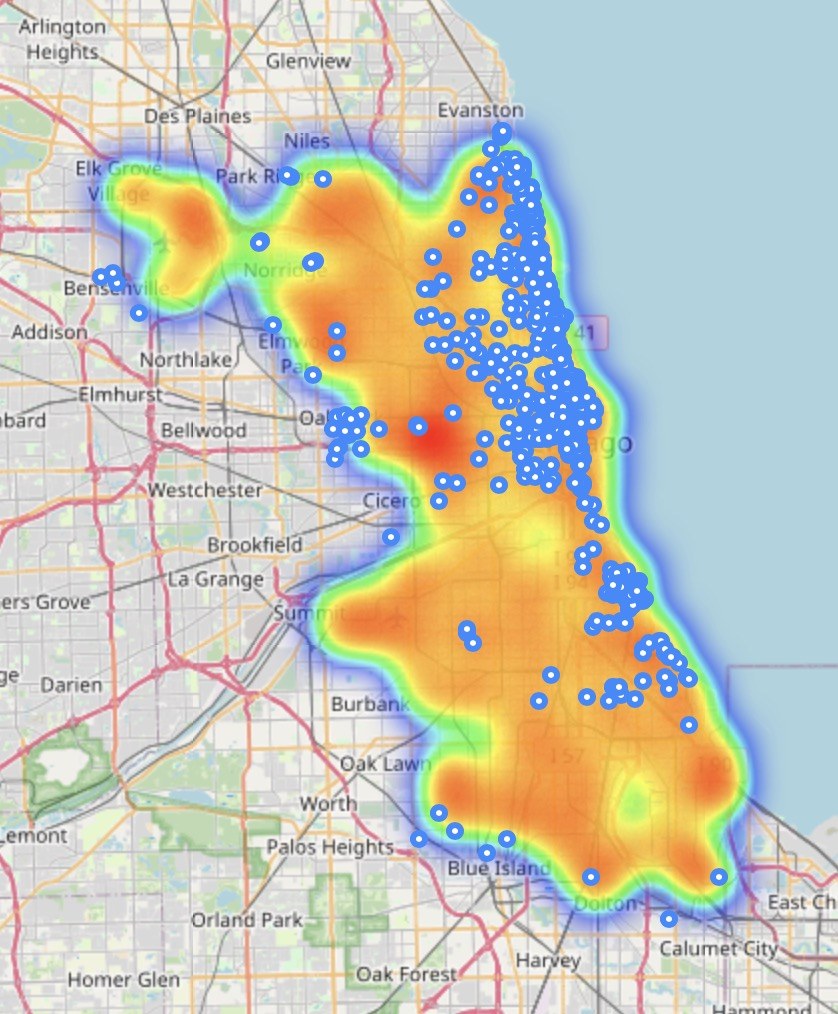
\includegraphics[height=6cm, width=4.8cm]{figs/intro_display.jpeg}
				\caption{Heat Map of Crime with Apartments Listed}
			\end{figure}
		\end{column}
	\end{columns}
\end{frame}


\section{Data Collection}

\begin{frame}
	\frametitle{Data Sources}
	\begin{itemize}
		\item \textbf{Apartments} (\url{www.apartments.com}) \newline Leading online apartment listing website; Offering renters access to information on more than 1,000,000 available units for rent.
		\item \textbf{Domu} (\url{www.domu.com/chicago/neighborhoods}) \newline The largest apartment listing site to focus on Chicago’s rental market. Founded by two brothers who grew up in rented apartments in Chicago.
		\item \textbf{Chicago's Open Data Portal} (\url{data.cityofchicago.org}) \newline Freely download the municipal data for your own analysis. Daily updated datasets with API provided.
	\end{itemize}
	\begin{figure}[H]
		\centering
		
\includegraphics[height=1cm, width=9cm]{figs/data_source.png}
	\end{figure}
\end{frame}


\begin{frame}
	\frametitle{Data: Scraping Apartments.com}
	\begin{itemize}
		\item Step 1: Collect all single property links in Chicago, IL\footnote{\url{https://www.apartments.com/chicago-il/}}
		\begin{itemize}
			\item Start from first listing page for Chicago $\rightarrow$ Collect all links within current page $\rightarrow$ Until last listing page
		\end{itemize}
		\item Step 2: Retrieve all information for a single property
		\begin{itemize}
			\item Property name, address, latitude, longitude, price, bedroom, bathroom, amenities
		\end{itemize}
		\item Step 3: Write data to csv file for later use
	\end{itemize}
	\begin{figure}[H]
		\centering
		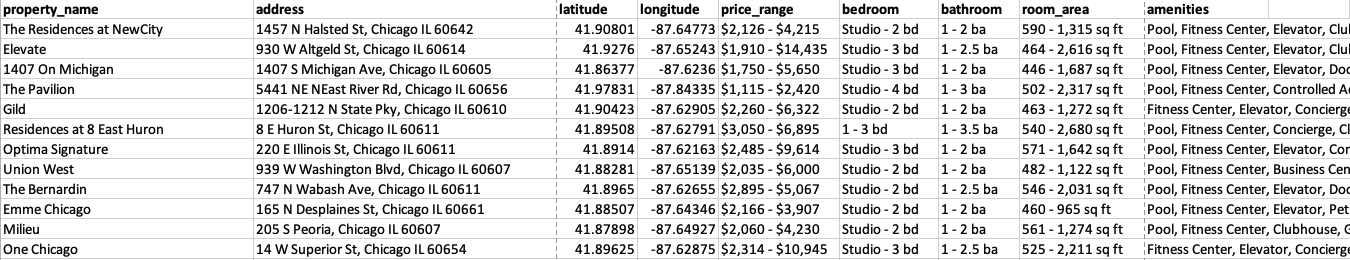
\includegraphics[height=2cm, width=10cm]{figs/apartmentsdata.png}
		\caption{Apartments.com Data}
	\end{figure}
\end{frame}

\begin{frame}
	\frametitle{Data: Crime}
	\begin{itemize}
		\item Chicago 2021 Crime Dataset
		\begin{itemize}
			\item Crime case number, case description
			\item Latitude, longitude (most important!)
		\end{itemize}
	\end{itemize}
	\begin{figure}[H]
		\centering
		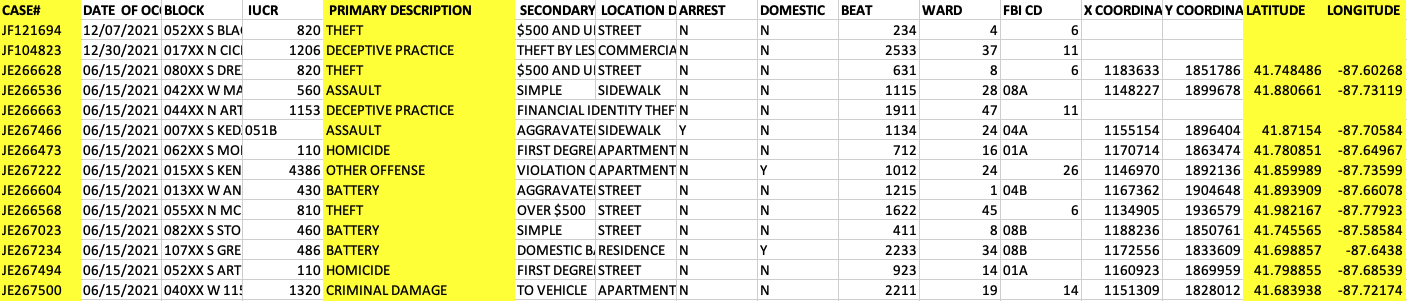
\includegraphics[height=2cm, width=9.5cm]{figs/crimedata.png}
		\caption{Chicago 2021 Crime Data}
	\end{figure}
\end{frame}



\section{Data Cleaning}

\begin{frame}{Data Cleaning}
    \begin{columns}
        \begin{column}{0.65\textwidth}
            \begin{itemize}
        \item Housing Data:
        \begin{itemize}
            \item Replace all zero values to "Not Available" for display purposes
        \end{itemize}
        \item Crime Data:
        \begin{itemize}
            \item Computing crime severity weights using \textit{Cambridge Crime Harm Index}
            \item Map each crime category to a weight score and add to data set
            \item Display crime severity weights in heat map
        \end{itemize}
    \end{itemize}
        \end{column}
        
    \begin{column}{0.35\textwidth}
        \begin{figure}[H]
			\centering
			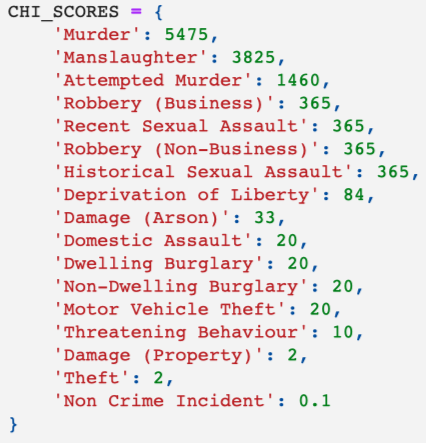
\includegraphics[height=4cm, width=3.5cm]{figs/chi_scores.png}
			\caption{CHI Score}
			\end{figure}
    \end{column}
    \end{columns}
    
    Side note: Cambridge Crime Harm Index is developed by UChicago Social Science Graduates!\footnote{\url{https://en.wikipedia.org/wiki/Crime_harm_index}} Paper available here.\footnote{\url{https://link.springer.com/article/10.1007/s41887-020-00043-2}}
\end{frame}



\section{Data Visualization}

\begin{frame}
	\frametitle{Data Visualization}
	\begin{itemize}
		\item Heat Map
		\begin{itemize}
		    \item Neighborhood crime in the last year
		    \item Weight depends on the type of crime
		    \item Our heat map is here\footnote{\url{https://github.com/cs-ssa-w22/final-project-none/blob/master/mapping.html}}
		\end{itemize}
		\item Housing Markets
		\begin{itemize}
		    \item Properties for rent
		    \item Information Displayed: Property name, address, bedroom, bathroom, amenities
		\end{itemize}
	\end{itemize}
	\vspace{0.8em}
	As it might be offensive and conflict interests of the property owners, we decided to create a heat map for security in the neighborhood rather than assign a security level score for each property.
\end{frame}




\section{Implications for Social Science}

\begin{frame}
	\frametitle{Implications for Social Science}
	\begin{itemize}
		\item Why Is It Important?
		\begin{itemize}
			\item Crimes in Chicago city is becoming more concerning. Safety will also be an important factor for tenants' decision making.
			\item Most of the apartment rental websites do not provide specific safety information due to conflict of interests.
			\item Heat map provides an intuitive observation to renters who concern about community safety. Users can get the features of properties by one clicking on the map
			\item Reduced the time and difficulty to access reliable rental data from multiple sites
		\end{itemize}
		\item How Is It Relevant to Social Science?
		\begin{itemize}
			\item Provide useful tools for future social science research on neighborhood security's influence on renters' decision making process
			\item Apply research in crime statistics to quantity community security status
		\end{itemize}
	\end{itemize}
\end{frame}

\begin{frame}
	\frametitle{Future Improvements}
	\begin{itemize}
		\item The whole web-scraping process takes about 1 to 2 seconds per page, resulting in a total of 15 minutes to write the csv file for apartments.
		\item Because housing data online is changing all the time, the current map can be outdated.
		\item The current interactive map is not very user-friendly. Future improvements can include richer information (e.g., property pictures, customer comments) and implement searching/filtering functions.
	\end{itemize}
\end{frame}

\section{Q\&A}

\begin{frame}
	\frametitle{Q\&A}
	\begin{center}
	    Any questions for us?
	\end{center}
\end{frame}


\begin{frame}{}
  \centering \Large
  Thank You!
\end{frame}




\end{document}